% !TEX root = ./xstream.tex

\section{Dynamic evaluation}

\textbf{Datasets}:

We use the same datasets as in HighDimension case in static setting. We create $10$ shuffled versions for each dataset. The datasets could either be shuffled randomly or it could be clustered in time. For the clustered shuffled, the input also includes a clustering percentage, that is how much percentage of anomalies should be clustered in time. We currently do not experiment with clustered in time datasets.

\textbf{Algorithms}
\begin{itemize}
\item{RS-Hash}: We use decay constant to be $0.015$, and use first $256$ samples to setup the $100$ components, and then compute AUC/AP over time.
\item{HS-Trees}:
\item{LODA}:
\end{itemize}

\textbf{Results}

\begin{figure*}[ht!]
    \centering
    \begin{subfigure}[t]{0.48\textwidth}
        \centering
        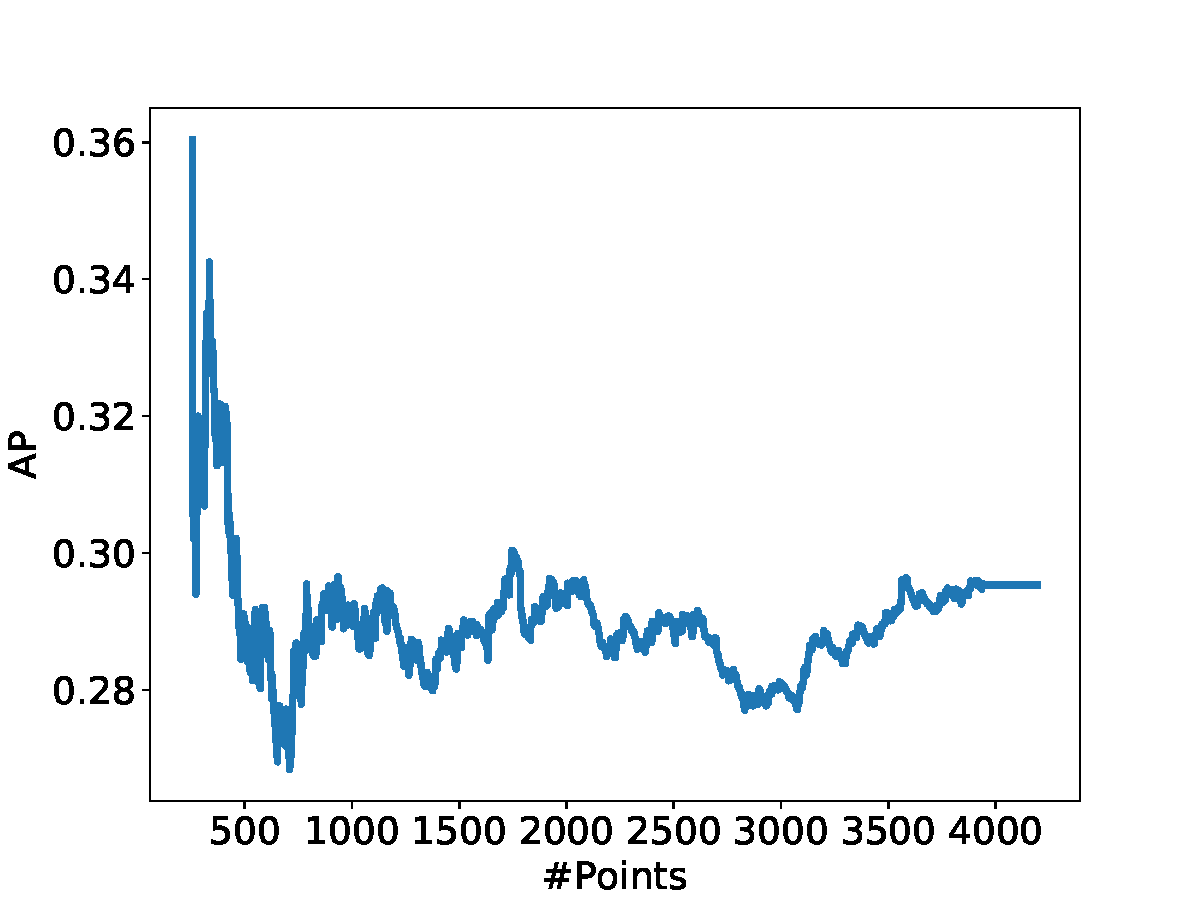
\includegraphics[width=\linewidth]{fig/streaming_baseline/letter-recognition.pdf}
        \caption{Low/Mid - dimensional dataset analysis}
    \end{subfigure}
    \hfill
    \begin{subfigure}[t]{0.48\textwidth}
        \centering
        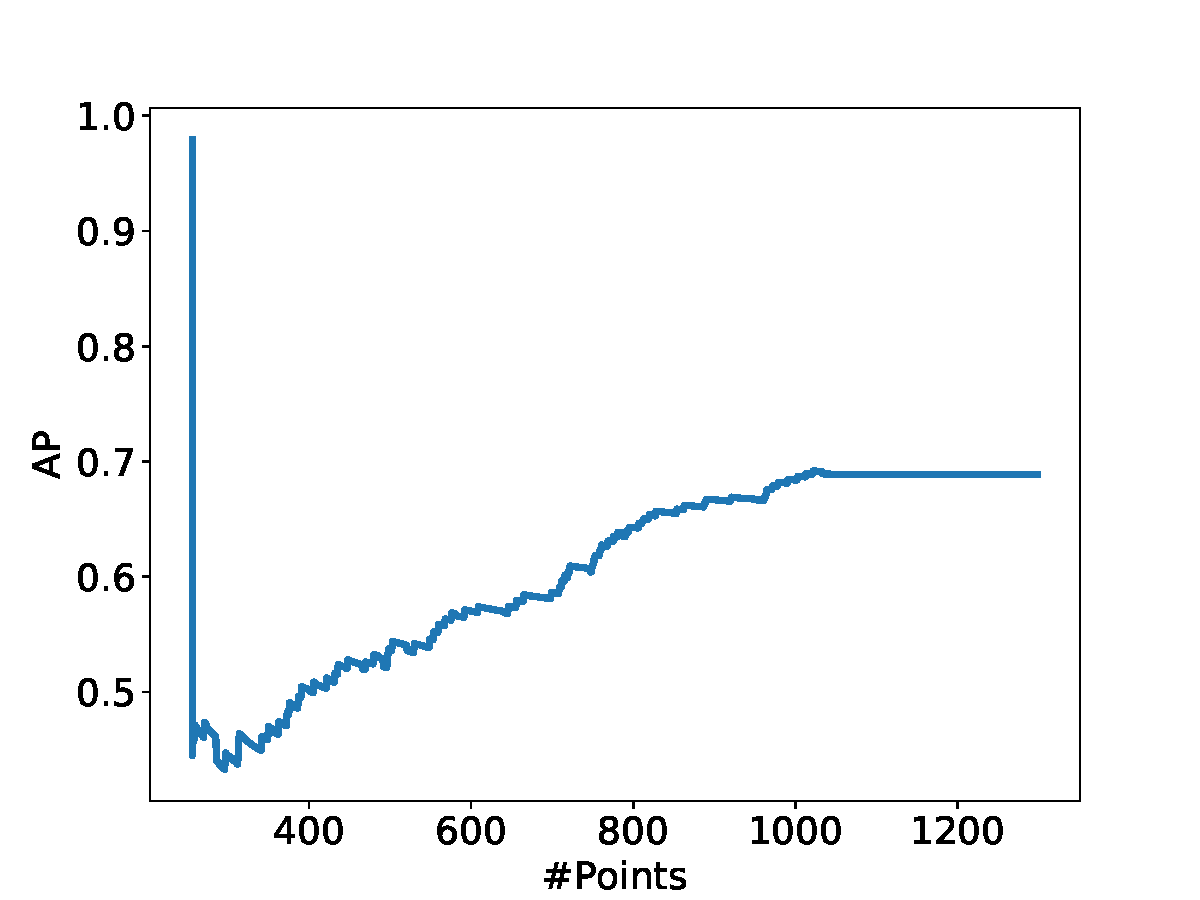
\includegraphics[width=\linewidth]{fig/streaming_baseline/madelon.pdf}
        \caption{High dimensional dataset analysis}
    \end{subfigure}
		\hfill
    \caption{AP for two of the baseline datasets over time, using RS-Hash Streaming Algorithm.}
\end{figure*}

\pagebreak
